\section{Results}

Using the \texttt{FEMPoissonSolver}, outlined in the previous section (see section \ref{sec:solver}),
we computed the solutions for a given problem and studied the convergence to the
exact solution for decreasing mesh spacings (mesh refinement).
The accuracy was tested for one, two and three dimensions and the convergence was good for each of them.

The problem solved was the Poisson equation with a sinusoidal source function
and homogenous Dirichlet boundary conditions.
In one dimension, the problem was:
\begin{align}
    -\Delta u = \pi^2 \sin(\pi x), \quad x \in [-1, 1],
\end{align}
with $u(-1) = 0$ and $u(1) = 0$.
The exact solution to this problem is:
\begin{align}
    u(x) = \sin(\pi x).
\end{align}

To solve this problem in two and three dimensions, the following $N$-dimensional variant of the same problem was used:
\begin{align}
    -\Delta u = N \pi^2 \prod_{i=1}^N \sin(\pi \vec{x}_i), \quad \vec{x} \in [-1, 1]^N,
\end{align}
where $N \in \mathbb{N}$ is the number of dimensions, the solution function $u$ is defined as:
$u: \R^N \to \R$, with the $N$-dimensional point $\vec{x} \in \R^N$ with its elements $\vec{x}_i \in \R : \ \vec{x}_i \in \vec{x}$ with $i \in \{1, ..., N\}$.
Also, the function $u$ is zero on the boundaries: $u(\vec{x}) = 0$ if for any entry $\vec{x}_i \in \vec{x}$,
it holds that $\vec{x}_i \in \{-1, 1\}$ for $i \in \{1, ..., N\}$.

This problem has the exact solution:

\begin{align}
    u(\vec{x}) = \prod_{i=1}^N \sin(\pi \vec{x}_i).
\end{align}

This test along with these sinusoidal functions are implemented in \texttt{TestFEMPoissonSolver}.

Different numbers of mesh vertices of powers of two were used in each dimension.
For a given number of mesh vertices $n$, the mesh spacing $h$ is given by:
\begin{align}
    h = \frac{2}{n - 1}.
    \label{eq:spacing}
\end{align}

The tolerance used in the CG algorithm was chosen to be $10^{-13}$.

In table \ref{table:sinusoidal_1d} the number of mesh vertices $n$ is given in the `Size column',
the `Spacing' is computed via equation \ref{eq:spacing}, the `Relative Error' is the relative error
of the computed solution compared to the analytical solution of the problem, the `Residue' is the
residue from the CG algorithm (see Algorithm \ref{alg:conjugate_gradient}) and the number of iterations
of the CG algorithm is given in the `Iterations' column.

\begin{table}[H]
    \centering
    \renewcommand{\arraystretch}{1.1}
    \small
    \begin{tabularx}{\hsize}{l l l l l}
        Size & Spacing              & Relative Error        & Residue               & Iterations \\ \hline
        4    & 0.6666666666666666   & 7.080989919320194e-09 & 4.440892098500626e-16 & 1          \\
        8    & 0.2857142857142857   & 1.249845927172312e-12 & 2.094764613337708e-15 & 1          \\
        16   & 0.1333333333333333   & 6.407420160623263e-16 & 5.325889242270741e-15 & 1          \\
        32   & 0.06451612903225806  & 1.779759178867111e-15 & 1.742186992884441e-14 & 1          \\
        64   & 0.03174603174603174  & 1.789223255831461e-16 & 6.654398136858673e-14 & 1          \\
        128  & 0.01574803149606299  & 3.503924460135148e-15 & 5.157582646417248e-14 & 2          \\
        256  & 0.007843137254901961 & 7.471370361275646e-15 & 8.253791443434346e-14 & 3          \\
        512  & 0.003913894324853229 & 2.094557289636767e-15 & 4.997105441592253e-14 & 5          \\
        1024 & 0.001955034213098729 & 2.178897100917102e-14 & 4.308783938700041e-14 & 177
    \end{tabularx}
    \caption{\texttt{TestFEMPoissonSolver} Output for the 1D sinusoidal problem.}
    \label{table:sinusoidal_1d}
\end{table}

\begin{figure}[H]
    \centering
    \includegraphics[width=12cm]{pictures/fem_convergence_sinus1d.png}
    \caption{1D Sinusoidal convergence}
    \label{fig:convergence_sinusoidal_1d}
\end{figure}

For one dimension, the solution converges with order 10 until it gets close to machine precision
(figure \ref{fig:convergence_sinusoidal_1d}).
This is much faster than anticipated and we assume it is
due to the smooth, periodic nature of the right-hand side chosen.
At the moment the solver only uses first-order Lagrangian finite element methods,
which are linear functions (see figure \ref{fig:1_lagrange_1d}).
There is a phenomenon for the trapezoidal quadrature rule, where it converges rapidly
when applied to analytic functions on periodic intervals \cite{trefethen_exponentially_2014}.

We think the convergence we are seeing for one dimension might be related to this phenomenon,
however, this was not investigated further but it might be interesting for future work.

\begin{table}[H]
    \centering
    \renewcommand{\arraystretch}{1.1}
    \small
    \begin{tabularx}{\hsize}{l l l l l}
        Size & Spacing              & Relative Error        & Residue               & Iterations \\ \hline
        4    & 0.6666666666666666   & 0.367835959800294     & 8.881784197001252e-16 & 1          \\
        8    & 0.2857142857142857   & 0.06877172889870629   & 2.054662609310059e-15 & 1          \\
        16   & 0.1333333333333333   & 0.01470558224055019   & 6.673718396468935e-15 & 1          \\
        32   & 0.06451612903225806  & 0.003428048120959612  & 1.226637297968919e-14 & 1          \\
        64   & 0.03174603174603174  & 0.0008291654851627174 & 2.735745689195284e-14 & 1          \\
        128  & 0.01574803149606299  & 0.0002039888701591884 & 1.157673913473065e-14 & 2          \\
        256  & 0.007843137254901961 & 5.059492109621404e-05 & 1.26186832683033e-14  & 3          \\
        512  & 0.003913894324853229 & 1.259908312652751e-05 & 7.423183529194849e-15 & 119        \\
        1024 & 0.001955034213098729 & 3.143610123038628e-06 & 3.751402450611288e-15 & 265
    \end{tabularx}
    \caption{\texttt{TestFEMPoissonSolver} Output for the 2D sinusoidal problem.}
    \label{table:convergence_sinusoidal_2d}
\end{table}


\begin{figure}[H]
    \centering
    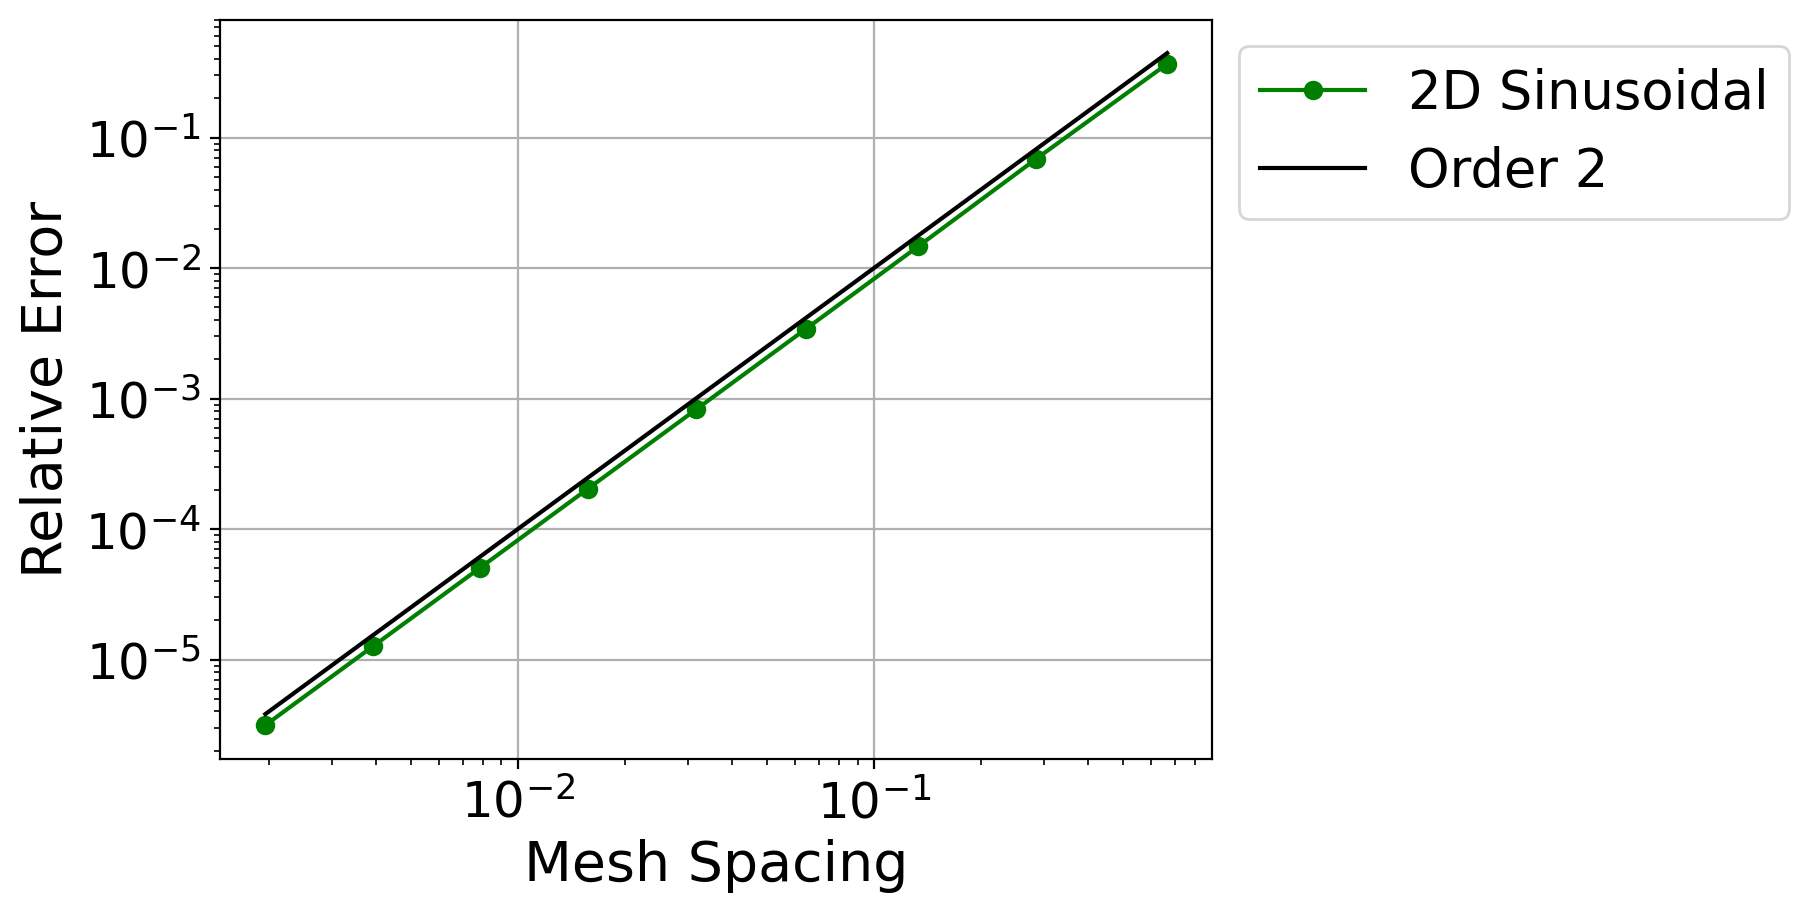
\includegraphics[width=12cm]{pictures/fem_convergence_sinus2d.png}
    \caption{2D Sinusoidal convergence}
    \label{fig:convergence_sinusoidal_2d}
\end{figure}

In two dimensions, the fast convergence from the one-dimensional study disappears and
it follows second-order convergence. This is the minimal rate of convergence expected for FEM
but it is to be expected for first-order Lagrangian finite elements.

\begin{table}[H]
    \centering
    \renewcommand{\arraystretch}{1.1}
    \small
    \begin{tabularx}{\hsize}{l l l l l}
        Size & Spacing             & Relative Error        & Residue               & Iterations \\ \hline
        4    & 0.6666666666666666  & 0.8709752261711512    & 1.368774871883577e-15 & 1          \\
        8    & 0.2857142857142857  & 0.1422730084945544    & 8.763930132546234e-15 & 1          \\
        16   & 0.1333333333333333  & 0.02962741863012481   & 1.814959731383155e-14 & 1          \\
        32   & 0.06451612903225806 & 0.006867847755836543  & 1.019648580795529e-14 & 1          \\
        64   & 0.03174603174603174 & 0.00165901848558236   & 1.623920791356438e-14 & 1          \\
        128  & 0.01574803149606299 & 0.0004080193515153442 & 3.485107117806992e-15 & 10
    \end{tabularx}
    \caption{\texttt{TestFEMPoissonSolver} Output for the 3D sinusoidal problem.}
    \label{table:sinusoidal_3d}
\end{table}


\begin{figure}[H]
    \centering
    \includegraphics[width=12cm]{pictures/fem_convergence_sinus3d.png}
    \caption{3D Sinusoidal convergence}
    \label{fig:convergence_sinusoidal_3d}
\end{figure}


In three dimensions, we get a very similar picture as in two dimensions.
We also observe second-order convergence.

Note: For three dimensions, the relative error was not computed for more than 128 mesh vertices (in each dimension)
due to the high computational load and the serial nature of this implementation.
